% THIS TEMPLATE IS A WORK IN PROGRESS

\documentclass{article}
\usepackage{graphicx}
\usepackage{hyperref}
\usepackage{fancyhdr}
\usepackage{float}

% FOR CODE
\usepackage{listings}
\usepackage{xcolor}

\definecolor{codegreen}{rgb}{0,0.6,0}
\definecolor{codegray}{rgb}{0.5,0.5,0.5}
\definecolor{codepurple}{rgb}{0.58,0,0.82}
\definecolor{backcolour}{rgb}{0.95,0.95,0.92}

\lstdefinestyle{mystyle}{
    backgroundcolor=\color{backcolour},   
    commentstyle=\color{codegreen},
    keywordstyle=\color{magenta},
    numberstyle=\tiny\color{codegray},
    stringstyle=\color{codepurple},
    basicstyle=\ttfamily\footnotesize,
    breakatwhitespace=false,         
    breaklines=true,                 
    captionpos=b,                    
    keepspaces=true,                 
    numbers=left,                    
    numbersep=5pt,                  
    showspaces=false,                
    showstringspaces=false,
    showtabs=false,                  
    tabsize=2
}

\lstset{style=mystyle}
% 

\fancypagestyle{firstpage}{%
  \lhead{CAP6610 Home Work 1 Report}
  \rhead{Akash Gajjar}
}

\begin{document}
\thispagestyle{firstpage}


\section{Implementation}

For the solution I have used Python version 3.8.10 . For operations related to linear algebra and to generate samples from Gaussian distribution with various parameters I am using \emph{numpy}, to plot the graphs from results I am using \emph{matplotlib}. I have implemented multiple functions to generate data and to perform Regression or Ridge Regression on the data and calculate the L2 distance between $\hat{\Theta}$ and $\Theta^{*}$. The function to perform the regression is implemented in such a way that if $N<K$ then it will perform Ridge Regression otherwise it will perform Regression using OLS.

\section{Graphs}

I have noticed that when $N<K$, sometimes we are not able to find the inverse of the matrix $X^{T}X$ or even if we are able to find the inverse of the matrix, the values are too high which results in L2 distance being very high. 

Below are some graphs for the L2 distance between $\hat{\Theta}$ and $\Theta^{*}$ for $N \in \{1 \dots 100\}$, $\lambda = 0.5$ and various values of $K$.

\begin{figure}[H]
  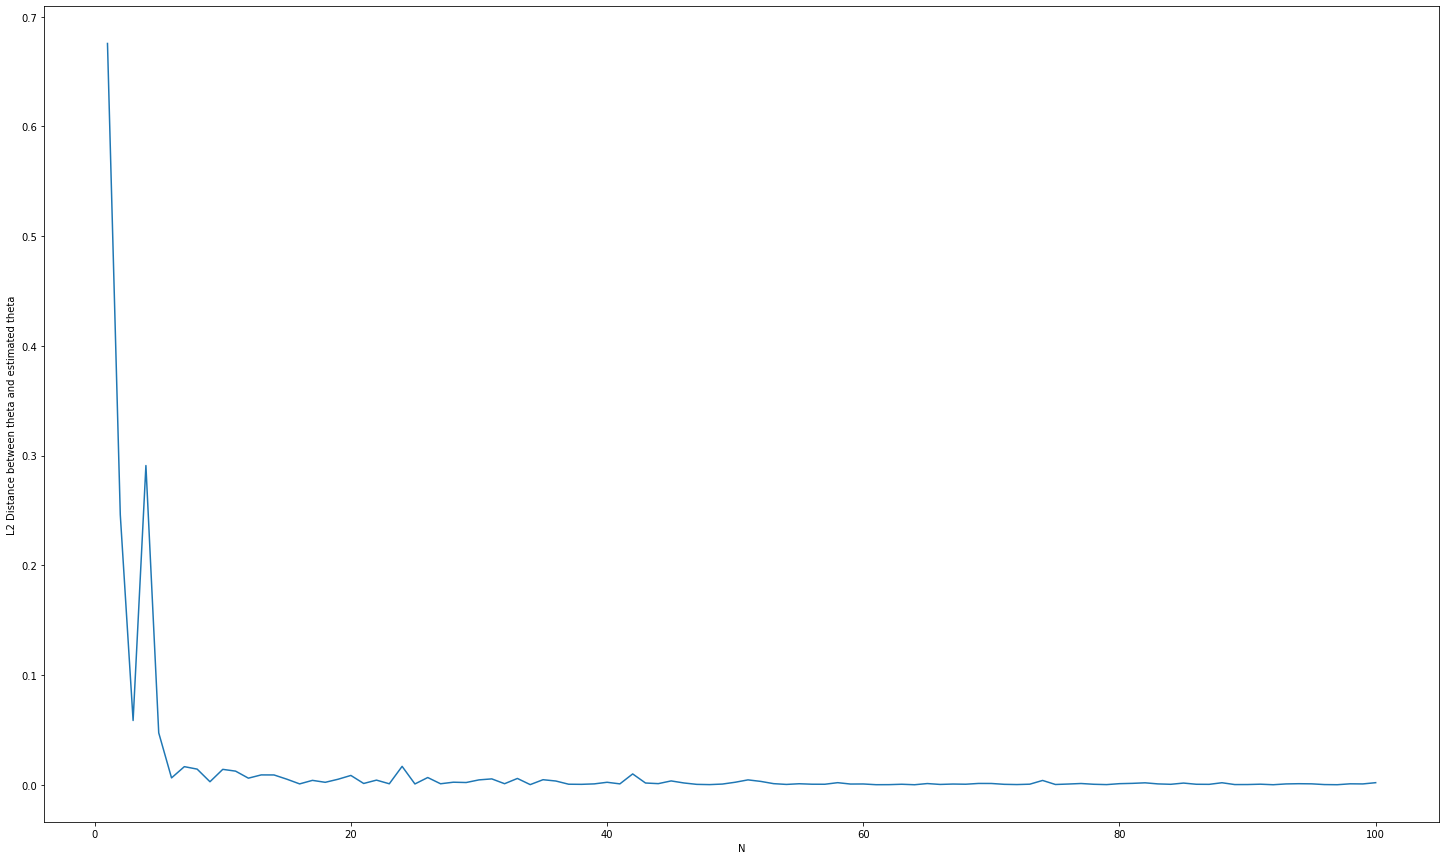
\includegraphics[width=\linewidth]{images/k-3.png}
  \caption{$K=3$}
\end{figure}
\begin{figure}[H]
  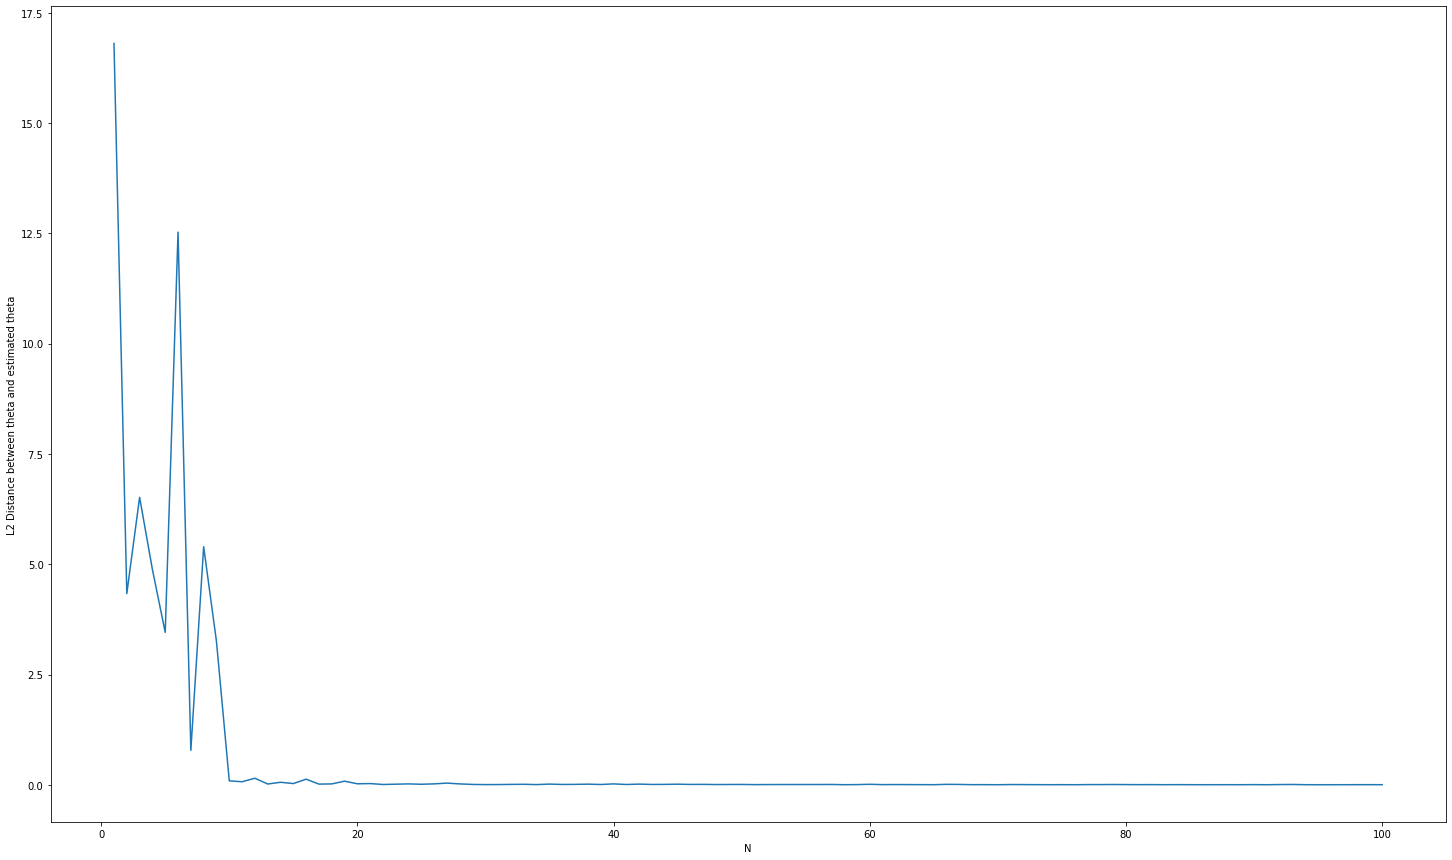
\includegraphics[width=\linewidth]{images/k-10.png}
  \caption{$K=10$}
\end{figure}
\begin{figure}[H]
  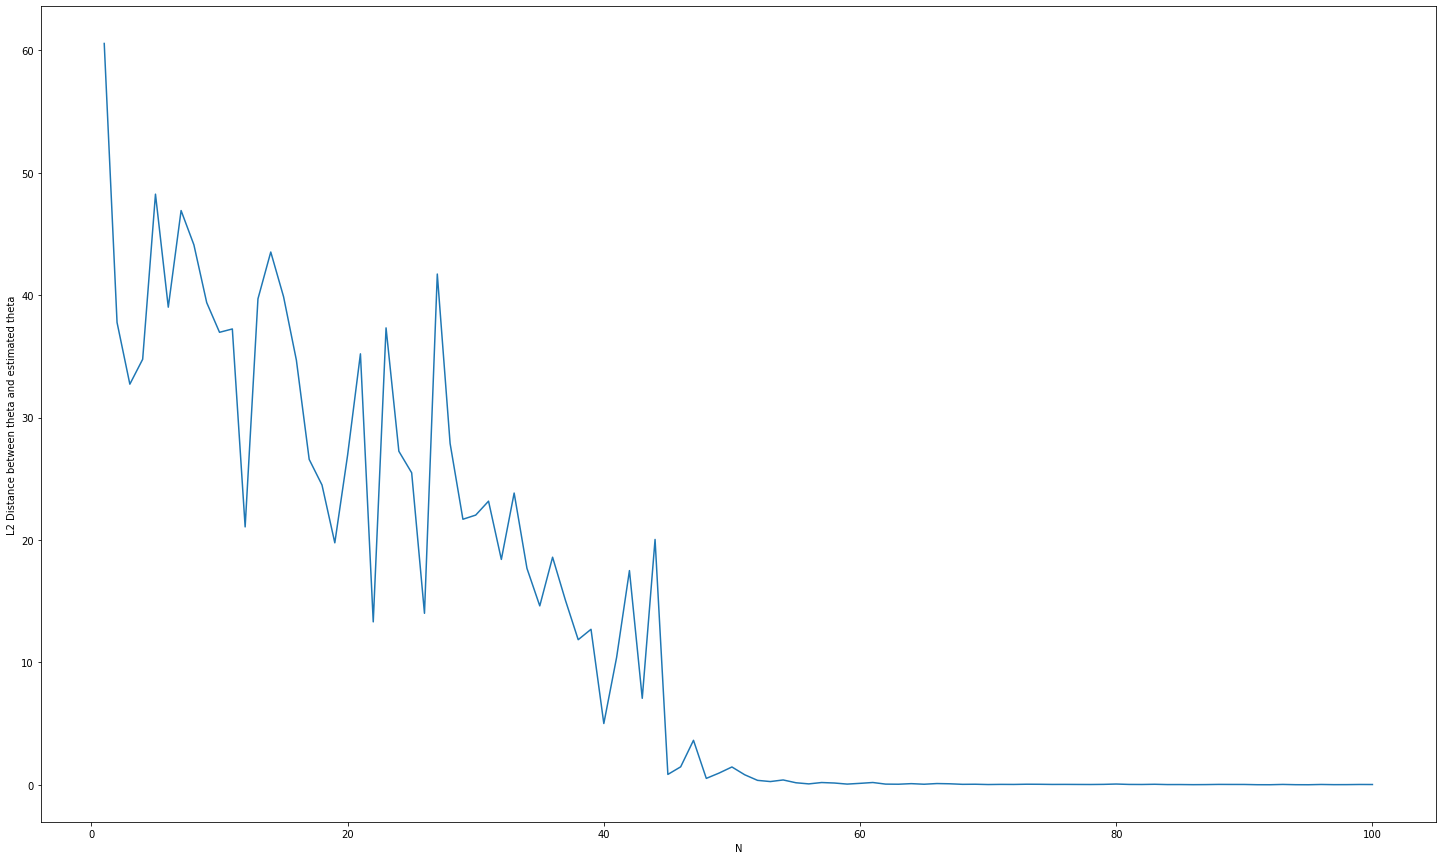
\includegraphics[width=\linewidth]{images/k-50.png}
  \caption{$K=50$}
\end{figure}
\begin{figure}[H]
  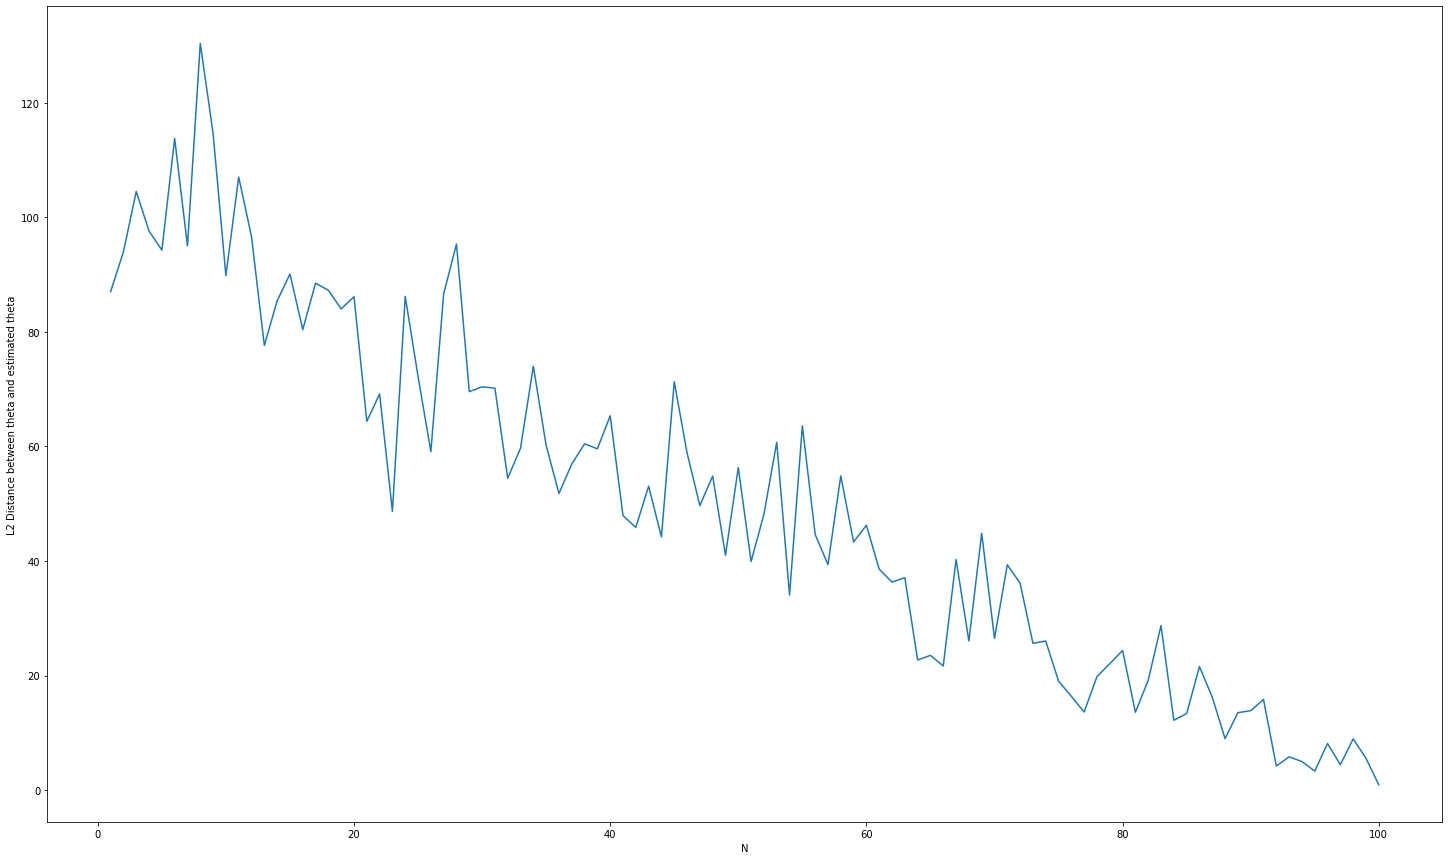
\includegraphics[width=\linewidth]{images/k-100.png}
  \caption{$K=100$}
\end{figure}

As you can see, when $N<K$, Ridge Regression is used and L2 distance is high and as soon as we have $N \geq K$, the L2 distance decreases significantly (almost zero).

\subsection{Ridge Regression}
To find out how does the L2 distance between $\hat{\Theta}$ and $\Theta^{*}$ vary with the value of $\lambda$, I fixed values of $N$ and $K$ as $1000$ and $50$ respectively and calculated the L2 distance for values of $\lambda$ in range $[0.001, 1.0]$ with $0.001$ step increments. Below is the plot for same.
\begin{figure}[H]
  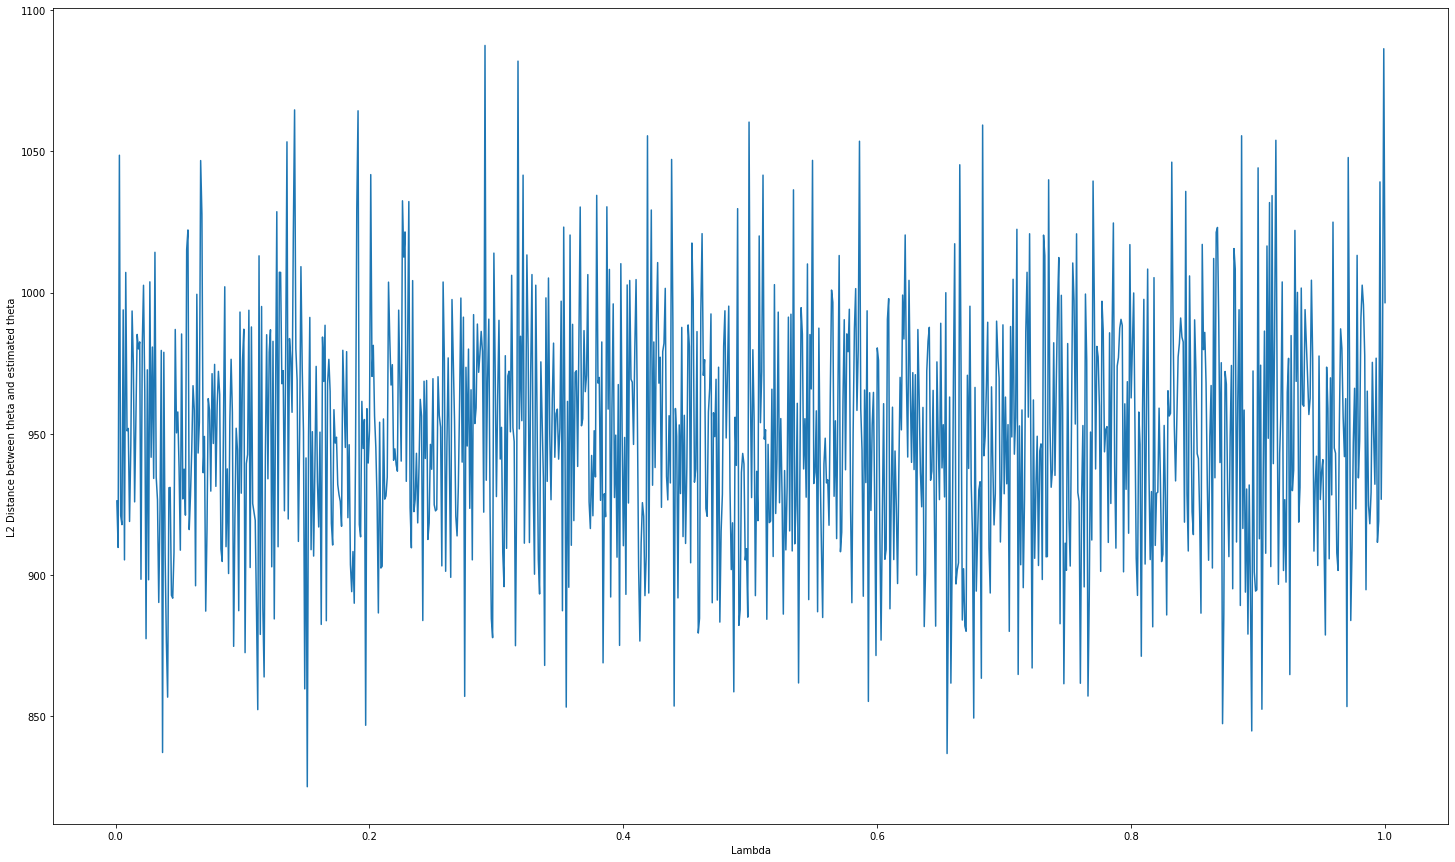
\includegraphics[width=\linewidth]{images/lambda.png}
  \caption{L2 distance between $\hat{\Theta}$ and $\Theta^{*}$ for various values of $\lambda$}
\end{figure}

It seems that there is no pattern in the L2 distance when we change the value of $\lambda$. I have tried large values of $\lambda$ as well but the graph was similar. 

\appendix
\section{Python Code}
\lstinputlisting[language=Python]{data.py}

\end{document}
